\begin{figure}[h]
    \centering
    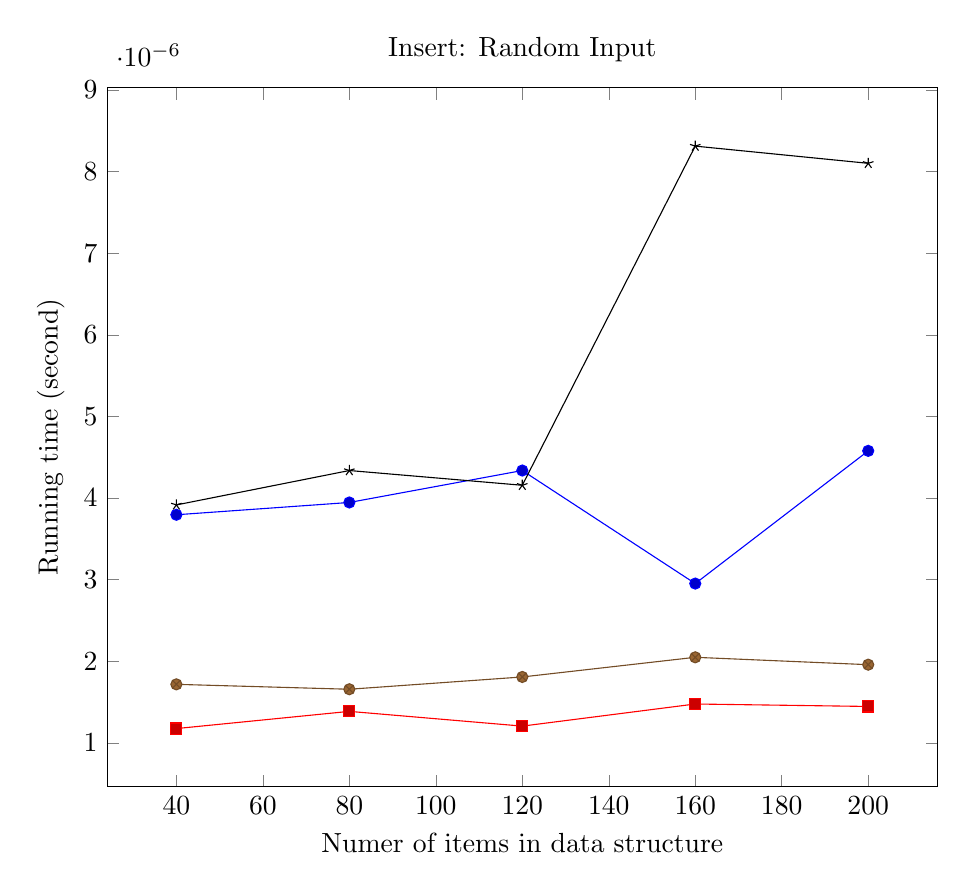
\begin{tikzpicture}
        \begin{axis}[
            xlabel={Numer of items in data structure},
            ylabel={Running time (second)},
            title={Insert: Random Input},
            width=\textwidth
        ]
		\addplot coordinates {
			(40, 3.794809243071085e-06)
			(80, 3.945396911446923e-06)
			(120, 4.336924849224103e-06)
			(160, 2.9515183001663877e-06)
			(200, 4.5778651186254234e-06)
		};
		\addplot coordinates {
			(40, 1.1745838133315427e-06)
			(80, 1.3854065490577148e-06)
			(120, 1.2047013470067348e-06)
			(160, 1.4757591500831612e-06)
			(200, 1.4456416164080992e-06)
		};
		\addplot coordinates {
			(40, 1.7166994194845256e-06)
			(80, 1.6564643521341412e-06)
			(120, 1.807052020510059e-06)
			(160, 2.04799228991151e-06)
			(200, 1.95763968888589e-06)
		};
		\addplot coordinates {
			(40, 3.915279377771606e-06)
			(80, 4.3369248492240374e-06)
			(120, 4.1562196471731445e-06)
			(160, 8.312439294346289e-06)
			(200, 8.1016165586199e-06)
		};
        \legend{}
        \end{axis}
    \end{tikzpicture}
    \caption{Average of 0 operations, benchmarked every 0, starting at 0.}
\end{figure}